\section{Introduction}

[TODO: Intention, hypotheses and results of the study]

Ethical, legal and social considerations are also part of my thesis.


Discussion centers on potential practical implications of the present results, as well as on prospects for future research.

\clearpage

\section{Background}

	\subsection{Motivation}
	
	E-learning providers are looking to improve the learning experience of their users and make progress as effective as possible. 
During a typical learning session each learner is subject to a range of volatile emotional states that help or hinder their learning success. 
Several factors and stimuli, both internal and external, can influence emotions. 
When we take this knowledge about emotions into account a new way to manage a learning session opens. We can incorporate this knowledge into learning sessions and provide a more appropriate task and interface for the learner.

The goal of the paper is to examine a relationship between the emotional aspect of a user interface in an e-learning system and its effect on the performance of the learner.


\begin{center}
	
\includegraphics[width=200px]{graphics/relation1.png}
\end{center}
 
There is strong evidence of the surrounding environment having an influence on emotion \cite{Johnson2000, Arockiam2013, Bertamini2013}. This includes, for example, an e-learning system on the screen in front of the learner. In a similar fashion several studies have shown a correlation between emotion and cognition (Section \ref{sec:emotion-cognition}).

\begin{center}

\includegraphics[width=300px]{graphics/relation2.png}
\end{center}

There is a logical argument of the existence of a transitive relation between these parameters, which could confirm the dependency of the edge variables. 
I.e. exposure to several interfaces each with a different emotional charge during an on-line lesson should lead to a difference in performance when working on the same task.
Insufficient research confirming this connection and explaining the effects has been published yet. 

In this paper I would like to explore to which extent the final parameter "learning success" can be influenced with the limited surface of contact that can be addressed through a learning interface on the screen.
	
		
	\subsection{Research basis} \label{sec:research}
	
	\toDo{about 10 pages of research}
	
	Information architecture and display types play an important role in learning comprehension, attention and learning success. \cite{McCrudden2017} describe the effects of different types of visual display on cognitive processing. They highlight the important aspects of visual guidelines, the basics of human understanding and  memory, as well a way to quantify those under processing efficiency. One of their conclusions is that "displays should be designed to support the selection of important information" \cite[p.633]{McCrudden2017}
	
	There is, however, a case to be made with respect to the same visual display that can be put forth in front of participants under differentiating emotional states. There is strong evidence that emotions play a role in information processing and, as a consequence, can have an effect on the resulting performance. Section \ref{sec:emotion-cognition} discusses closer existing research supporting a connection between emotion and cognition.
	
	Evidence also suggests that specific emotion can be caused through the use of emotional design features. Section \ref{sec:emotional-design-features} proposes a set of general rules for emotional design based on previous research.
	
	A recent study \cite{Haaranen2015} suggests that wrong choice of emotional design patterns can yield contra-productive results. It reports lover concentrations levels in the experiment group compared to control group using abstract graphics when learning object-oriented programming (OOP). Due to their choice of presentation and the topic or learning, the material has not been perceived as serious and a such became distracting.
		
		\subsubsection{Emotion theory} \label{sec:emotion-theory}
		
		To understand how emotion acts as a mediator to e-learning and learning in general it is important to see what emotion is and what causes it.
		
		From a biological perspective \textbf{emotion} is a collection of responses triggered from parts of the brain to the body or other parts of the brain. A series of such responses results in an \textit{emotional state} and is defined by changes within the body. \cite{Damasio1998}
	
		Emotion is caused by various internal and external events. Internal events can be immune activity or hormone changes. External events - observed or felt in the outside world - contribute additionally to internal ones. People have do direct access to the causal connections of emotions and little to no control of them. One can undergo a change of emotion without knowing why. \cite{Russell2003}
		
		Russell proposes that at the base of any emotion the experienced states are either good or bad, energized or enervated. As such these are the two "core affects" that govern our perception, behavior and cognition. \cite{Russell2003}. 
		
		There are individual differences of average levels of core affect and its responsiveness to stimuli due to the genetic differences. \cite{Russell2003}
		
		Over the years of psychological research, models of emotion have taken a range of representations. 
		A popular approach is the "Circumplex Model of Affect" \cite{Russell1980}, where emotions can be summarized and laid out in a two-dimensional space. The horizontal axis describing the "pleasure" (futher used as valence) dimension. The vertical axis - the arousal dimension.
		
		Assumptions in this paper are largely based upon the "Circumplex Model". I classify possible emotional states into four quadrants which are mutually discrete. To simplify, they are be labeled for further reference as shown in figure \ref{fig:valence_arousal_model}):
		\begin{enumerate}
			\item[Q1:] Angry (Quadrant 1)
			\item[Q2:] Happy (Quadrant 2)
			\item[Q3:] Sad (Quadrant 3)
			\item[Q4:] Relaxed (Quadrant 4)
		\end{enumerate}
		
		
		\begin{figure}
			\begin{center}
				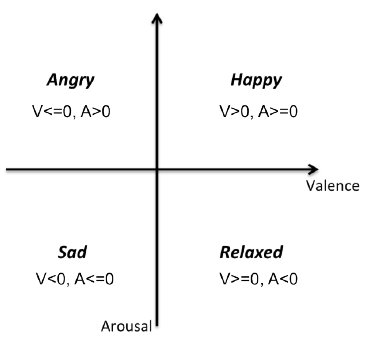
\includegraphics[width=150px]{graphics/Valence-Arousal-model-showing-the-quadrants-of-the-four-emotion-tags-used-in-this_W640.jpg}
				\caption{Valence Arousal Model \cite{Song2013} \label{fig:valence_arousal_model}}
				
			\end{center}
		\end{figure}
		
		
		\toDo{[TODO]: summarize Valence-Arousal model and explain 4 groups}
		
		\subsubsection{Emotion and cognition} \label{sec:emotion-cognition}
		
		A 2004 cognitive neuroscience study \cite{Dolcos2004} scanned participants brain activity, while rating emotional pictures. The study makes several relevant conclusions. First, that different parts of the brain show stronger activity when exposed to positive compared to negative stimuli. Second, that high arousal stimuli lead to greater successful encoding activity, or in other words - rate of recall, than neutral stimuli. 
		
		In other words, brain response is different for arousing stimuli of positive valence compared to negative valence. Furthermore memory is mediated, in part by both - valence and arousal levels. It provides basis to the assumption that variation on both dimensions is necessary to adequately reflect effects within e-learning context. Study design in \ref{sec:study-design} depends heavily on this assumption.
		
		
		
		\subsubsection{Emotion and visual interface}
		
		\cite{Desmet2007} demonstrates in their research that physical objects can cause significant emotional response and that modifying design attributes can successfully contribute to creating of desired response.
		Both physical objects and digital visuals are, in essence, interfaces. Both can cause an emotional response \citationneeded Digital interfaces are extremely flexible to experimentation and modification at low cost.
		
		
		Good sources:
		\cite{Valdez1994} - effects of color on emotions
		\cite{Plass2014} - Emotional design in multimedia learning: Effects of shape and color on affect and learning
		\cite{Swasty2017} - Does Color Matter on Web User Interface Design?
		\cite{Pert1996} - Color Research and Its Application to the Design of Instructional Materials
		\cite{Tekirdag2015} - The Effect of Colour on Human Body and Psychology
	
	\subsection{Hypotheses}
	
		\paragraph{Hypothesis 1.} Two different interfaces do not result in a significant difference in emotional response
		\paragraph{Hypothesis 2.} Performance of participants on memory and creativity tasks, as measured by selected study design parameters, during the experiment is equal with interface 1, and with interface 0.

\section{Approach and Methods}

To facilitate the study I make assumptions about the medium in which e-learning is usually conducted. Based on previous research (\ref{sec:research}) I define study design parameters and a set of target variables that are measured and evaluated.

	\subsection{Medium}
	
	The study is to be conducted online under a "real-life" scenario. This means, that the experiment is to be run in a browser-capable web-application runnable on modern personal computers. Like most e-learning software the  application used in the study is browser-based and usually used in a user's home or public venue.
	
	\subsection{Study design} \label{sec:study-design}
	
	Goal of the current study is to determine emotional response difference to provided emotional design implementation (Interface 1) compared to the control group that is provided with a stricter desaturated design (Interface 0). Differences include use of color, shapes, language, font style, interaction responsiveness, animation. The similarities or - constant variables - across both interfaces include any accessibility features and general usability heuristics, such as contrast ratio level, size and placement of elements on a screen. Further details of the emotional design aspects, that are included in the current implementation are shown in section \ref{sec:emotional-design-features}
	
	Participants of the study are not informed about the existence of another interface as a variable but rather only made aware about being emotionally influenced by preconditioning and that their performance during the experiment is being measured. Abundance of timers throughout the test highlight the time sensitivity of the tasks to the participant.
	
	The experiment can be outlined and split into following steps:
	
	\begin{enumerate}
		
		\item[0.] \textbf{Clustering:} Each participant is assigned an interface version (1 of 2) and the preconditioning group (1 of 4) at random before first load of the application.
		
		\item \textbf{Emotional report:} A short emotional self-reporting questionnaire (SAM \ref{sec:selfeval}) is used to acquire initial valence and arousal ratings
		
		\item \textbf{Preconditioning:} Each participant is shown a set of emotional images and preconditioned to be in one of 4 states:
			\textbf{1}: Positive valence / high arousal;
			\textbf{2}: Negative valence / high arousal;
			\textbf{3}: Positive valence / low arousal;
			\textbf{4}: Negative valence / low arousal;
			
		Choice of stimuli and their presentation is described further in chapter \ref{sec:preconditioning}
			
		\item \textbf{Emotional report:} Emotional self-reporting questionnaire (SAM \ref{sec:selfeval}) to validate, whether preconditioning has had a sufficient and expected effect on the participant.
		
		\item \textbf{Experiment 1:} Slightly modified classic memory game. The participant is presented with a grid of tiles, each tile containing an image. During 10 seconds at the beginning of the experiment all tiles are open to allow to memorize the images. After which all images are hidden. Only 2 tiles can be opened at any one time. Once both tiles of the same image are open they are marked as solved. The goal is to solve all tiles. Detailed description in section \ref{sec:memory}
		
		\item \textbf{Experiment 2:} Remote Associates Test (RAT). A generalized creativity test developed by Mednick \cite{Mednick1962} in 1962. Each participant is presented with a number of word sets. Each set consists of 3 words that are shown to the participant and one target word that is hidden from the them. The target word is semantically connected to all 3 visible words. Detailed description in section \ref{sec:creativity}
		
		\item \textbf{Emotional report:} A second emotional self-reporting questionnaire (SAM \ref{sec:selfeval}) is used to establish, whether and which effect tasks and interface have had on the participant's emotion.
		
		\item \textbf{Demographic data:} Final step adds additional personal context data for each participant through a questionnaire to complement data analysis (discussed in \ref{sec:demographics}).
		
	\end{enumerate}
	
	\subsection{Preconditioning sequences} \label{sec:preconditioning}
	
	\paragraph{Finding a preconditioning sequence}
To facilitate emotional conditioning I selected a specialized sequence containing images with a corresponding emotional charge.
Each sequence contains 21 to 39 \todo{more precise} images with each displayed for about 5 seconds.

Each subject is assigned one of four preconditioning sequences. Each sequence is aimed to condition the subject into one of the 4 quadrants, described though a valence-arousal emotional model. To simplify we will label (\ref{fig:valence_arousal_model}) them as:
\begin{enumerate}
	\item Angry (Quadrant 1)
	\item Happy (Quadrant 2)
	\item Sad (Quadrant 3)
	\item Relaxed (Quadrant 4)
\end{enumerate}


\begin{figure}
\begin{center}
	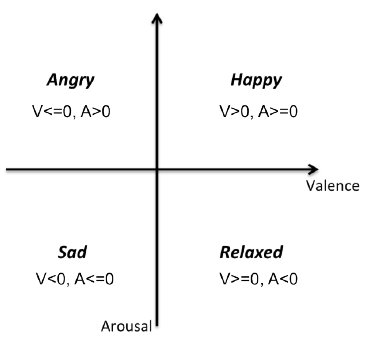
\includegraphics[width=150px]{graphics/Valence-Arousal-model-showing-the-quadrants-of-the-four-emotion-tags-used-in-this_W640.jpg}
	\caption{Valence Arousal Model \cite{Song2013} \label{fig:valence_arousal_model}}
	
\end{center}
\end{figure}

There are several emotional image data-sets available for academic purposes such as GAPED \cite{Dan-Glauser2011}, OASIS \cite{Kurdi2017}, IAPS \cite{Lang1997} and NAPS \cite{Marchewka2014}. While NAPS is offering the highest realism and quality of images, the range images seems to cover "sad" and "happy" to a less pronounced degree. In general, strong negative valence values are accompanied with high arousal values across all analyzed data-sets. Causing sadness is a challenging task. In current preconditioning sequences I am using the \textbf{OASIS} database. It has relatively wide spread of emotions compared to other sets.

Keeping in mind the need for a clear separation between groups in terms of their emotional state into account, I limited emotional images to moderately strong stimuli values, thus avoiding extreme reactions and unrealistic emotional states. It can be assumed that in most cases, people who attend e-learning lessons will have moderate levels of emotional charge. It is important to note that quadrant 1 - angry and quadrant 2 - happy has a more pronounced representation in emotional databases due to an easier and more prevalent stimuli availability. As such quadrant 1 and quadrant 2 have stronger stimuli compared to quadrant 3 and 4. It is expected that there will be a significant difference between emotion ratings of participants across these groups.

It is understood that the e-learning interface under real conditions will only cause mild-to-moderate changes to a mood.


\begin{figure}
	\centering
	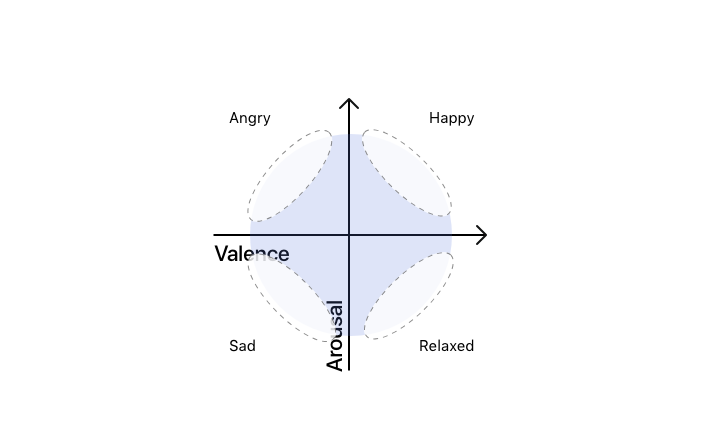
\includegraphics[width=0.7\linewidth]{graphics/Valence-Arousal-Model-1.png}
	\caption{Focus levels of emotional states on valence arousal model}
	\label{fig:valence-arousal-model-2}
\end{figure}

Illustration \ref{fig:valence-arousal-model-2} highlights with dashed outline areas the target arousal and valence values

	
	\subsection{Emotional Design Features} \label{sec:emotional-design-features}

Under real conditions it can be expected that the e-learning interface will cause mild-to-moderate changes to a mood.
	
	\toDo{write about emotional design, rewrite citation blocks below}
	
	\cite{Arockiam2013}: Personality traits play a role in connection with User Interface Design for performance
	
	\cite{Brom2018}: Anthropomorphisms/colors consistently increased learning outcomes.
	
	\cite{Le2018}: Compared to the participants in the neutral design group, the participants in the positive emotional design group performed better on a subsequent retention test
	
	\cite{Mayer2014} For the enhanced group, the graphics were redrawn to render the host cell as a red face with expressive eyes (registering surprise, fear, and sickness at various stages in the process), and the virus as a blue face with fierce eyes and with a green dot at the end of each of the blue tentacles surrounding the virus face. The enhanced group performed better than the control group on a subsequent learning test
	
	Studies shown in section \ref{sec:research} strongly suggest a connection between user interface and learning performance. They analyze performance and presentation based on concrete content examples. In present study I attempt to generalize the findings to a more universal set of guidelines that is not specific to certain content and can be applied to any e-learning topic.
	
	\clearpage

\paragraph{Developing a high performing interface}

There is a multitude of studies that analyze user interface design and user emotion. In following I will summarize them in respect to UI features tailored towards high performance

\paragraph{Literature review}

A paper by L. Arockiam et al \cite{Arockiam2013} describes that, based on previous research and their own findings optimal ui can be achieved based on a person's personality traits. We will limit ourselves to a universal set of changes that should evoke high arousal, positive valence and therefore have an effect on learning outcome, rather than look for their preference. Nevertheless it is worth mentioning...

Color - PHYSIOLOGICAL

Wilson (1966) reported higher GSR measurements for red as opposed to green, and Nourse and Welsh (1971) reported higher GSR readings for violet than green. Using 24 male college students as subjects and saturated samples of red, yellow, green, and blue as stimulus materials, Jacobs and Hustmyer (1974) found that red was significantly more arousing than either yellow or blue, and green more than blue. Using 40 undergraduate students as subjects, Jacobs and Suess (1975) found that red and yellow resulted in higher anxiety state scores than blue or green when measured by the StateTrait Anxiety Inventory. Bloomer (1976) also reported that red increases heart rate. There appears to be some evidence that spectral extremes, especially red, cause greater arousal than mid-spectral colors. This may relate to the fact that wavelengths at the extremes of the spectrum, such as red and violet, focus at different points in the eye than wavelengths at the middle of the spectrum. \cite{Pert1996}

Color - PSYCHOLOGICAL

The selected order of preference was: (1) blue, (2) red, (3) green, (4) violet, (5) orange, (6) yellow. This selection agreed with the average rankings of color preference among 21,060 subjects reported in earlier investigations. The order was the same for all races and for men and women with one exception. Men chose orange over yellow whereas women chose yellow over orange. \cite{Pert1996}

no significant differ- ences between men and women or between subjects of different races.\cite{Pert1996}

girls of all ages preferred higher value, brighter, colors as compared to boys (Child, et al., 1968) \cite{Pert1996} (study among school age children from 1 to 12 grade)

Results on the evaluation scale supported the general preference for cool colors(bl~e and green) as compared with warm colors(red and yellow) and agree with previous findings by Adams and Osgood (1973) that red is a potent color while gray and black have low potency. \cite{Pert1996}

In a color-effectiveness study conducted at Fort Monmouth, typical army training procedures were used with 11 different television lessons (Kanner and Rosenstein, 1960). No significant
differences were found in learning between
monochrome and colored versions \cite{Pert1996}

Schaie (1966) pointed out that color prefer-
ences vary from individual to individual and relate to personality. \cite{Pert1996}

(so far black and white and color has not yielded any significant difference in learning) but "colored mate- rials are preferred by learners." \cite{Pert1996}

1972: those who viewed colored transparencies had had a more positive attitude toward transparencies than \cite{Pert1996}

In a research study on color coding, Lamberski and Dwyer (1983) concluded that color is an attention-getting device that can provide measurable effects on learning that cannot be accounted for by words and labels. \cite{Pert1996}

Search Tasks: 
gain in efficiency, indicated by decreased search time, with codes of up to five colors \cite{Pert1996}

Color was found to be useful in grouping information

color versions resulted in higher recognition- memory scores (immediate recognition memory test)\cite{Pert1996}

as the variable of visual complexity increases, so does the degree of recall. (Berry (1991a)) \cite{Pert1996}

The key factor relating to color and cogni-
tive learning seems to be that it is of value when it emphasizes relevant cues, is used as a coding device, or when it is a part of the con- tent to be learned (Dwyer and Lamberski, 1982- 83; Levie, 1973; Pruisner, 1993; Wedell \& Alden, 1973). \cite{Pert1996}

Non-objective Measures

(Scanlon, 1970). Scanlon suggests that the color versions (Grey Cup football game) create emotional effects that detract from attention to details.







Colors at the ends of the spectrum, red and
violet, seem to result in greater arousal, and
colors in the middle of the spectrum, yellow,
green, cyan, seem to be best for discriminating
detail. \cite{Pert1996}
	
	\subsection{Experiments}

		\subsubsection{Experiment 1: Short term Memory} \label{sec:memory}
		
		Memory Experiment 
		
		[TODO:] Describe basis of the experiment
		
		[TODO:] describe activity logging for EXP1 here?
		
		\paragraph{Performance variables:} \label{sec:memory-parameters}
		
		[TODO:] measuring performance of this experiment
		
		\subsubsection{Experiment 2: Creative thought} \label{sec:creativity}
		
		A generalized creativity test developed by Mednick \cite{Mednick1962} in 1962 requires the participant to perform creatively. They are "asked to form associative elements into new combinations by providing mediating connective links" \cite[p. 226]{Mednick1962}. This test is called Remote Associates Test or RAT.
		It is developed in such a way that completing it does not require prior knowledge of any particular subject. 
		
		Participants are shown a set of three stimulus words from mutually remote associative clusters. Their task is to provide the mediating link between them. The link must be of an associative manner, rather than one that applies additional logic or inferences. Figure \ref{fig:exampleratset} shows an example of such word-set with a solution.
		
		A possible limitation is knowledge of language and cultural influence. Mednick himself states that RAT problems rely on "verbal associative habits could reasonably be assumed to be familiar to almost all individuals that have been brought up in this (USA) culture". The originally presented 30-element list of problems can have a certain degree of dependency on the cultural linguistic habits. For present study additional steps are taken to exclude possible problems due to these effects. 
		
		To minimize the limitation of language knowledge participant is required at the beginning of the study to comply with conditions, which contain (among others) "advanced English knowledge" (Appendix \ref{itm:participation_requirements}). After the tests the participants are asked to state whether or not they are native English speakers and to confirm their English knowledge level.
		
		\begin{figure}[h]
			\centering
			\includegraphics[height=0.3\textheight]{graphics/Example_RAT_Set}
			\caption{Example remote associate word-set "Cottage, Swiss, Cake"}
			\label{fig:exampleratset}
		\end{figure}

		The current experiment uses a further development of the original Mednick's remote associate test presented by Bowden in a 2003 paper. Bowden et al. \cite{Bowden} have developed 144 sets of remote associate problems with an additional constraint. The solution word has to not only be related to the triad of stimulus words but additionally each of them should form a commonly used compound word or two-word phrase with the solution word. The solution word can build either the first part or the second part of the phrase.
		
		Bowden's word-sets are a subset of all possible remote associate problems and have been alternatively described as "compound word problems".
		
		\toDo{longer description of what Bowden proposes with some quotes}
		
		Some \textbf{20} of a set of 144 compound remote associate sets are taken from \cite{Bowden}. Some of the easier (top solving percentage rate among 30-second threshold test participants, published by Bowden) word-sets are selected for present experiment while avoiding certain colloquialisms related to a location. As a result, these 20 word-sets should be challenging although solvable to a wide array of people from different backgrounds. Table \ref{table:1} presents a list of the used RAT items in the current study. The difference in time taken to solve a problem act as indicator for performance. (\ref{sec:creativity-parameters}).
		
		\paragraph{Experiment details}
		
		The participant is informed about the rules and what is expected from them:
		
		\begin{displayquote}
			"You will see three stimulus words. Attempt to generate a fourth word that is related to each stimulus word. When combined with each of the stimulus words will build a word pair that is a common compound word or phrase. The goal is to find a solution as fast a possible
			
			After 30 seconds you will see 2 words appearing as hints on the screen, only one solution is correct.
			The first 3 are practice sets and will allow you to train. During practice we will give you a hint after 10 seconds"
		\end{displayquote}
	
		The participant is shown 3 practice tasks which allow them to get used to the interface and the dynamics of the task. As most of the participants are remote and unsupervised it is important to give an intuitive set of instructions and avoid any variation due to unclear interface or task.
		
		\begin{figure}[h]
			\centering
			\includegraphics[width=0.7\linewidth]{"graphics/creativity versions"}
			\caption{Example screen showing both versions of interface during creativity experiment}
			\label{fig:creativity-versions}
		\end{figure}
	
		After 3 practice tasks, participant clicks on "Start Experiment" before solving 20 items defined in the set. An example preview of both interface screens with the three stimulus words and an input for the answer is displayed in figure \ref{fig:creativity-versions} 
		
		Upon appearance of each word-set a timer starts tracking the time to enter a word.
		Stimulus words appear with a 200ms delay from timer start and 50ms delay between each word appearing. The appearance animation takes 300ms. All items are completely visible at 600ms mark, with the first word in the left-to-right direction completely visible and static at 500ms after timer start. 500ms can be discounted from the time it takes to solve a problem (Effectively participants have 29.5 seconds to solve a problem).
		
		\paragraph{Appearance of Hints}
		
		Each word-set has a 30 second limit to solve a problem. After time is expired a block with 2 hint words \ref{fig:hint-buttons} appear. One of which is the correct solution to the problem, another is a false solution. It is semantically clear which solution is correct, upon reading it the participant is expected to experience the "aha!" effect mentioned in \cite[p.634]{Bowden} with a reference to previous research. Choosing the wrong answer, once the time expires can be a hint that the participant is not paying attention.
		
		After hints appear, the problem is not any more counted as solved by the participant. 
		
		\textit{Hints appearance can be delayed.} Due to a person requiring time to type the answer on a keyboard it is assumed the answer is known once the first letter of the word is written in the field. There is a 3000ms grace delay to type each additional character. Grace delay accounts for typing speed and is deemed sufficient for most persons. Erasing a character is considered as typing (and resets the counter) unless the first letter of the input is erased. Once the delay is passed or the first letter erased the hints appear and the problem is marked as unsolved. Time of the first letter being typed is considered an objective point of time that a participant figures out the answer to the problem. The time of first letter is always within 30 seconds of appearance of the word-set.
		
		\begin{figure}
			\centering
			\includegraphics[width=0.3\linewidth]{"graphics/Hint buttons"}
			\caption{Hints after time allowed for solving a problem is elapsed}
			\label{fig:hint-buttons}
		\end{figure}
		
		
		Once all items are solved they are directed to the next page of the interface.
				
		\paragraph{Activity logging} \textit{Experiment 2} activity is specified based upon generalized logging of activity in e-learning described in \ref{sec:activitylog}
		
		A generic action emitter triggers an action when either of the following happens:
		
		\begin{itemize}
			\item Click on button to start practice
			\item Click on button to start live experiment
			\item Event when word set appears on screen
			\item Event when word set is guessed correctly
			\item Event when word set is guessed incorrectly
			\item Event when word set has expired (hint words appear)
		\end{itemize}
	
		Each event object contains system status information and context information about current words visible.

		\paragraph{Performance variables} \label{sec:creativity-parameters}
		
		\begin{enumerate}
			\item Aggregated solving speed: seconds taken to solve a problem on average
			\item Non-aggregated solving speed: seconds taken to solve each problem
			\item Idea generation ratio: how many attempts (including false ones) are taken within the time limit on average
			\item Success rate: Number of problems solved successfully
			\item Frustration/Negative-attention: Amount of false choices after \textit{Hint Word} suggestion appears as ratio to Hint Word suggestion answers.
		\end{enumerate}
	
		\toDo{elaborate about the measures and reasoning behind them}


	\subsection{Means of emotional self-evaluation} \label{sec:selfeval}
	
	

% \todo[inline, size=\tiny]{'Valence and Arousal evaluation techniques'}


	
	[TODO:] Describe Valence and Arousal evaluation techniques
	
	SAM , AS, Affect Grid \cite{Russell1989} (the same guy who created the circumplex model 9 years prior)
	
	Due to effort constraints of the participants it is important to achieve a simple, yet accurate reading of their emotions. In the context of this study self-evaluation is a means to validate results, of Hypothesis 1. I chose to rely on the proven SAM (Self-Assessment Manikin) method \cite{Bradley1994} to quickly allow users to assess their emotions on a dual 9 point scale.
	
	\subsection{Demographic data and supplemental information} \label{sec:demographics}
	
	As final step of the study each participant fills out a demographics questionnaire to add context data and help with analysis. There are 4 questions:
	
	\begin{enumerate}
		\item Gender \\ \ [Male / Female]
		\item Age \\ \ [18-24 / 25-29 / 30-34 / 35 - 44 / older]
		\item Is English your native language? \\ \ [yes / no]
		\item What is your level of English knowledge? \\ \
			[Beginner  / Intermediate / Advanced / Fluent]
		\item Occupation: \\ \ [High school student / Undergraduate Student / Graduate Student / Doctorate / Professional or Working]
		\item Email (optional)
	\end{enumerate}

	Gender (Question 1) allows to uncover difference in performance or response due to gender. Possible disparities are expected to be observed as described in \ref{sec:preconditioning}

	The age groups (Question 2) are taken in accordance with suggestions provided by the Standard International Age Classifications \cite{UN1982} with slight modifications to exclude ages below 18. Further the study would focus on ages up to 44. Ages above 44 could potentially skew results due factors not considered by present study. Primary focus audience lies between ages of 18 and 34.
	
	Native speakers (Question 3) might potentially score higher on the creativity task due to cultural influence of using colloquial expressions. This assumption is challenged during data analysis in section \ref{sec:data-validity}
	
	Question 4 is used to validate the requirement of at least an "advanced" proficiency in English. Participant choosing anything lower could suggest either invalid data or problems with the creativity task due to language issues. In this case participant is considered for removal. \todo{evaluate this claim}
	
	Occupation is asked simply for additional context into the participant.
	
	Final email field allows the user to enter their email address for participation in the raffle and complies with the motivational promise at the beginning of the experiment.

	\subsection{E-learning activity logging} \label{sec:activitylog}
	%To assess performance of subjects several measurements are taken during the test, these differentiate between the 2 experiments.
	
	\toDo{[TODO:] Describe general approach to recording actions and recording approach for this study.}
	
	Each participant is defined as a \textit{user}. Each user is assigned a session for each new started experiment. 
	
	To assess the performance of participants continuous measurements are taken during a session of the experiment. A general approach is an event-based system where each \textbf{action} from the \textit{user} or the \textit{system} is emitted to the database. A differentiation is established between a "click" action that is initiated by the user and an "event" action that is initiated by the system environment.
	
	For correct attribution at the moment when action is emitted it contains: 
	\begin{itemize}
		\item userID, sessionID, timestamp (unique key)
		\item name of active screen
		\item type of action (\textit{event} or \textit{click})
		\item context information such as global system state and dependent values of current active screen
	\end{itemize}

	Finally, for system actions (events) \textbf{name of event} is provided. For user actions (clicks) a target of the click is provided.
	
	%A session is defined on the scope of single e-learning module and contains user metadata as well as emotional state of the learner.

	

		
		\paragraph{Technical implementation}
		
		Upon requesting the page a user-token is generated and assigned to each participant. This token is saved as a cookie for future reference and visitor matching. Only one successful experiment is allowed per participant due to 
		Each experiment further contains a session object with its attributes. 
		
		"[location]\_[action]\_[result]"
		
		\toDo{[TODO:] describe how tracking is implemented, storage and analysis for current study}
		
		Action tracking is managed by a dedicated module that communicates with the database storage API. Each event sent to the Database is complemented with a timestamp and user data. An action object with usual fields is described in listing \ref{lst:db_object}


	\begin{listing}[H]
		\begin{minted}{json}
			{
			"first": "second1"
			}
		\end{minted}
		\caption{Database Object Fields}
		\label{lst:db_object}
	\end{listing}

\toDo{specify object}

		
		\paragraph{xAPI adaptation} - 
		
		\toDo{[TODO Optional:] explore adaptability and possible constraints}

\section{Study implementation}

\paragraph{Participant sourcing} 
This study includes participants attained through multiple sources:
\begin{itemize}
	\item{Local university:} On-site supervised experiments were conducted on a limited scale to facilitate a clean sample of participants and uncover problems during the study
	
	\item{Local workplace:} On-site semi-supervised experiments are conducted on a limited scale in Berlin area in Germany to facilitate a more diverse sample while keeping controlled environment conditions, similar to university experiments.
	
	\item{Social media:} Remote participants are invited to participate in unsupervised experiments on their own. Channels such as social media, interest groups and university mailing lists are used.
	
	\item{Mechanical turk:} MTurk is one of popuar web services to source participants. Previous research has shown that it can be considered a reliable platform for conducting objective studies. MTurk participants receive monetary compensation for participation \cite{Buhrmester2011a}. Mturk participants are excluded from motivation with a chance on winning a voucher prize (they do not see the field and information box about it), instead regular participant reward through MTurk is used.
	
\end{itemize}

Local and social media experiments provided additional motivation of participation with the promise of a chance to win a 20 Euro Amazon-voucher.

\paragraph{Technical implementation} is guided by the requirement to run the study in a browser on a personal computer. React.js is selected as a library of choice due to it's favorable characteristics to creating an environment that supports 2 themes and global settings in a scalable way. 


React's unidirectional data flow allows clear behavior path between application data and visual representation. In particular, it becomes possible to adjust the theme of the interface and propagate in-place an alternative style and visual rules throughout the application without losing current state. Additional benefits of this approach are discussed in section \ref{sec:further-research} in the context of an emotionally aware interface.

\begin{figure}
	\centering
	\includegraphics[width=1\linewidth]{"graphics/App Architecture"}
	\caption{Component based architecture with emotion control mechanism}
	\label{fig:app-architecture}
\end{figure}

Current implementation contains a minimal proof of concept of a way to enable e-learning interfaces to be complemented with emotional data. On one side data about the nature of the task, as discussed by \cite{Haaranen2015} and acknowledged in section \ref{sec:research}. On the other side about the emotional state of the user, either through ambient and body-sensors, or by other means.

Through this architecture (as shown in figure \ref{fig:app-architecture}), it is possible to develop an interface that responds to emotional and task contexts with an appropriate interface.

\section{Results and Evaluation}

	\subsection{Collected data}
	
	[TODO:] Describe data preparation, how many people participated, demographics data, distributions.
	[TODO:] Show general statistical data
	
	\subsection{Validity} \label{sec:data-validity}
	
	\paragraph{Native speakers} 
	\textbf{H\textsuperscript{0}:}  Native speakers (Question 3) do not score differently on the creativity task due to cultural influence 
	
	\paragraph{Females} 
	\textbf{H\textsuperscript{0}:} Female reaction to Q2 Preconditioning is not different than male
	
	\subsection{Evaluation}
	
	[TODO:] Here describe how evaluation was done
	
\section{Conclusions}

	\subsection{Hypothesis 1}
	
	[Note:] H1 should be checked in the context of the whole app
	
	\subsection{Hypothesis 2}
	
	[Note:] H2 should be checked for each task separately

\section{Further research and implications of the study} \label{sec:further-research}

\subsection{Ethical, legal and social implications}

[TODO]

\section{Notes}




